\documentclass[12pt,a4paper, xcolor=table]{article}
\usepackage{graphicx}
\usepackage[utf8]{inputenc}
\usepackage{eurosym}
\usepackage[spanish,es-tabla]{babel}
\usepackage[left=2cm, right=2cm, top=2cm, bottom=2cm]{geometry}
\usepackage{afterpage}
\PassOptionsToPackage{hyphens}{url}\usepackage{hyperref}
\usepackage{subfig}
\usepackage[table,xcdraw]{xcolor}
\usepackage{cite}
\usepackage{url}
\usepackage{changepage}

\usepackage{imakeidx}
\newcommand\blankpage{%
    \null
    \thispagestyle{empty}%
    \addtocounter{page}{-1}%
    \newpage}
\renewcommand*\contentsname{Índice: }

\makeindex
\let\olditemize\itemize
\def\itemize{\olditemize\itemsep=0pt}

\begin{document}
\setlength{\parindent}{0pt}
\begin{titlepage}
        \centering
        
\includegraphics[width=0.75\textwidth]{img/logo_uc3m.jpg}\par\vspace{2cm}
        {\huge\bfseries Práctica 3 \\ Sistemas Borrosos\par}
        \vspace{0.5cm}
        {\scshape\Large Inteligencia Artificial en las Organizaciones\par}
        \vspace{1.5cm}
        {\scshape\Large Grupo 83-1\par}
        \vspace{1.5cm}
        {\Large\itshape Miguel Gutiérrez Pérez\par}
        {\Large 100383537@alumnos.uc3m.es \par}
        \vspace{1cm}
        {\Large\itshape Mario Lozano Cortés\par}
        {\Large 100383511@alumnos.uc3m.es\par}
        \vspace{1cm}
        {\Large\itshape Alba Reinders Sánchez\par}
        {\Large 100383444@alumnos.uc3m.es\par}
        \vspace{1cm}
        {\Large\itshape Alejandro Valverde Mahou\par}
        {\Large 100383383@alumnos.uc3m.es\par}
        \vspace{5mm}
        {\large GitHub: \textbf{\textit{\href{https://github.com/Pheithar/InteligenciaArtificialOrganizaciones}{InteligenciaArtificialOrganizaciones}}}}
        \vfill

% Bottom of the page
        {\large \today\par}
\end{titlepage}

\tableofcontents

\newpage

\section{Introducción}

Los sistemas borrosos hacen uso de la \textit{Lógica Difusa}, que es una técnica del área de la inteligencia artificial que permite la inclusión de conceptos humanos vagos para resolver problemas\cite{fuzzy}.

\vspace{2mm}

Es un tipo de lógica que reconoce más que valores de verdadero o falso, pues permiten decir el grado de verdad o falsedad de distintas variables, puediendo llegar a usar variables lingüísticas\cite{fuzzygame}.

\vspace{3mm}

Este tipo de sistemas expertos intenta abordar los problemas tal y como lo haría un humano: en términos relativos, y en grados de pertenencia. Estos conceptos vagos son los que usan normalmente los humanos a la hora de razonar.

\vspace{3mm}

Los dos problemas que se plantean están fuertemente relacionados con el \textit{COVID-19}. Se trata de crear dos sistemas borrosos capaces de decidir, por un lado \textbf{cuándo hay que confinar una población} y, por otro, \textbf{cuándo hay que realizar una prueba PCR a un paciente}. Estos problemas pueden ser solucionados a través de sistemas borrosos porque las variables involucradas, tanto de entrada como de salida, pueden ser transformadas en el grado de pertenencia a una clase concreta.

\vspace{4mm}

Es importante remarcar que los datos que se han usado para la resolución de la práctica, a falta de contactos con expertos, se han tomado de distintas fuentes del \textit{Ministerio de Sanidad}\cite{poblacion, paciente} de España. Para poder complementar los sistemas borrosos, ya que requerían de más información, se han interpretado estos valores por los autores. Por tanto, sería necesario realizar una revisión a través de expertos, ya sean médicos, virólogos o epidemiólogos que puedan confirmar o corregir los valores y franjas introducidas.

\vspace{3mm}

Sí es cierto que el criterio de realización de pruebas PCR, a pesar de que pueda llegar a ser distinto en cada país, está muy bien acotado y definido. Esto ha faciltado la realización de su sistema borroso.

\vspace{2mm}

No es así en el caso del sistema borroso para decidir si confinar o no una población, puesto que no está explicado ni expuesto correctamente en ningún documento público. A pesar de que el \textit{Ministerio de Sanidad}\cite{poblacion} incluya unas directrices que informen de los rangos de valores para diferentes niveles de riesgo, no indica a partir de cuales de esos valores se ha de confinar.

\vspace{4mm}

Para resolver los problemas propuestos se utiliza la herramienta \textit{Fuzzy Logic Toolbox (FLT)} de MATLAB debido a que permite manejar fácilmente los principales aspectos cuando se quiere crear un sistema borroso.

\newpage

\section{Contexto de la práctica}

La lógica difusa es muy útil cuando se desea representar y operar con conceptos que tengan imprecisión y sirve cuando hay ciertas partes del sistema a controlar que son desconocidas y no pueden medirse de forma fiable.

\vspace{3mm}

Los sistemas borrosos, al igual que numerosas técnicas de IA, puede ser aplicada sobre muchos tipos de problemas diferentes, como, por ejemplo, en diagnóstico médico, intercambio de acciones de bolsa, optimización de centrales de energía, e incluso el manejo automático de un helicóptero\cite{fuzzy}.

\vspace{2mm}

Un caso que puede resultar especialmente llamativo es el uso de la lógica difusa para controlar un NPC (\textit{Non-Playable Characters}) en un videojuego\cite{fuzzygame}. Este pequeño caso de estudio intentaba y conseguía demostrar la eficacia y simpleza que resulta la aplciación este tipo de soluciones a entornos dinámicos.

\vspace{2mm}




\section{Sistema borroso: Confinamiento}
De manera inicial se plantea el desarrollo de un sistema borroso que decida la conveniencia o no de confinar a una población en función de una serie de parámetros o variables de entrada al sistema que se detallarán en la subsiguiente sección.

\subsection{Variables de entrada}
Tras un estudio meticuloso de las variables relevantes en la tarea que se trata de resolver y mediante el apoyo en la información oficial proporcionada en el ámbito de la \textit{Estrategia Nacional para la COVID-19 del Gobierno del Reino de España} [3] se determinan como relevantes la siguiente relación de variables.

\begin{itemize}

    \item \textbf{Incidencia acumulada de casos diagnosticados en 14 días} (IA-14): Casos confirmados en 14 días *100.000 / número de habitantes. Sus posibles valores son: \textit{Muy Bajo}, \textit{Bajo} \textit{Medio }, {\textit{Alto}} y {\textit{Muy Alto}}. La figura~\ref{IA-14} muestra los intervalos de cada uno de los posibles valores de forma gráfica.

    \begin{figure}[!h]
      \centering
      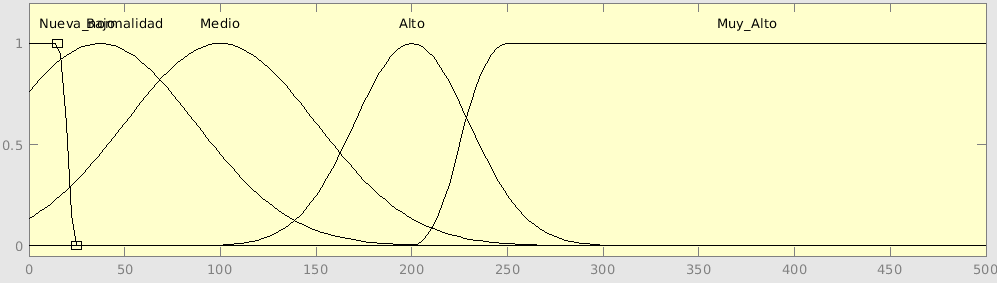
\includegraphics[width=300px]{img/ia_ac_14.png}
      \caption{IA-14}
      \label{IA-14}
    \end{figure}

    \item \textbf{Incidencia acumulada de casos diagnosticados en 7 días} (IA-7): Casos confirmados en 7 días *100.000 / número de habitantes. Sus posibles valores son: \textit{Muy Bajo}, \textit{Bajo} \textit{Medio }, {\textit{Alto}} y {\textit{Muy Alto}}. La figura~\ref{IA-7} muestra los intervalos de cada uno de los posibles valores de forma gráfica.
    
    \begin{figure}[!h]
      \centering
      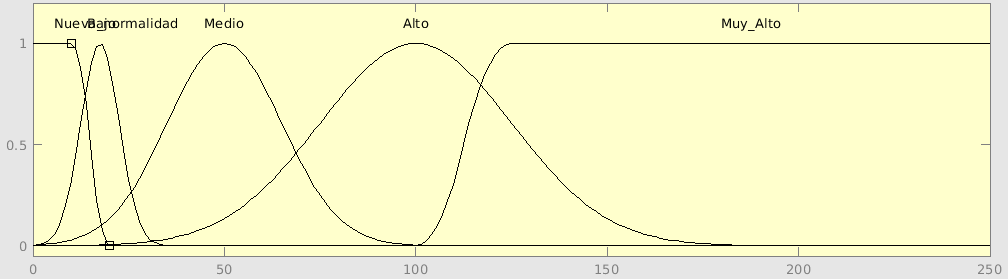
\includegraphics[width=300px]{img/ia_ac_7.png}
      \caption{IA-7}
      \label{IA-7}
    \end{figure}

    \item \textbf{Incidencia acumulada de casos diagnosticados en Incidencia acumulada de casos con 65 o más años diagnosticados en 14 días} (IA-14 65): Casos >= 65 años confirmados en 14 días *100.000 / número de habitantes >= 65 años. Sus posibles valores son: \textit{Muy Bajo}, \textit{Bajo} \textit{Medio }, {\textit{Alto}} y {\textit{Muy Alto}}. La figura~\ref{IA-14 65} muestra los intervalos de cada uno de los posibles valores de forma gráfica.
    
    \begin{figure}[!h]
      \centering
      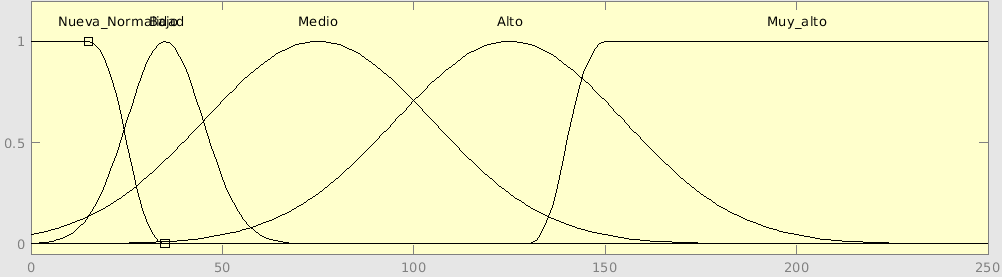
\includegraphics[width=300px]{img/ia_65_14.png}
      \caption{IA-14 65}
      \label{IA-14 65}
    \end{figure}

    \item \textbf{Incidencia acumulada de casos diagnosticados en Incidencia acumulada de casos con 65 o más años diagnosticados en 7 días} (IA-7 65): Casos >= 65 años confirmados en 7 días *100.000 / número de habitantes >= 65 años. Sus posibles valores son: \textit{Muy Bajo}, \textit{Bajo} \textit{Medio }, {\textit{Alto}} y {\textit{Muy Alto}}. La figura~\ref{IA-7 65} muestra los intervalos de cada uno de los posibles valores de forma gráfica.
    
    \begin{figure}[!h]
      \centering
      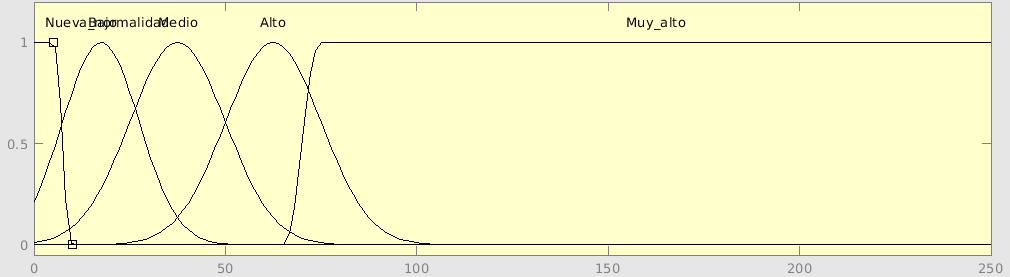
\includegraphics[width=300px]{img/ia_65_7.png}
      \caption{IA-7 65}
      \label{IA-7 65}
    \end{figure}

    \item \textbf{Positividad global de las PDIA (Prueba Diagnóstica de Infección Activa) por semana} (PDIA): Número de pruebas con resultado positivo en 7 días *100 / Número de pruebas realizadas en 7 días. Sus posibles valores son: \textit{Muy Bajo}, \textit{Bajo} \textit{Medio }, {\textit{Alto}} y {\textit{Muy Alto}}. La figura~\ref{PDIA} muestra los intervalos de cada uno de los posibles valores de forma gráfica.
    
    \begin{figure}[!h]
      \centering
      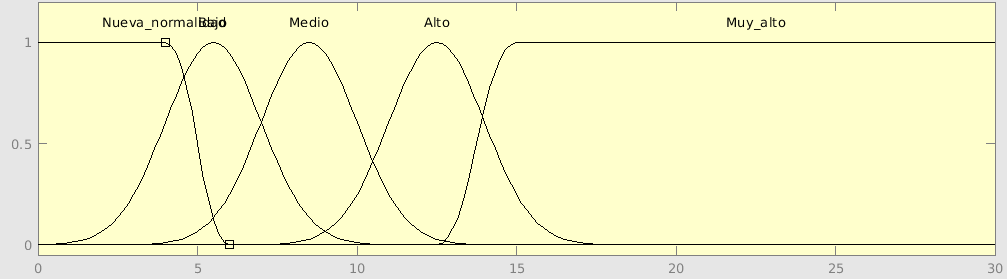
\includegraphics[width=300px]{img/PDIA.png}
      \caption{PDIA}
      \label{PDIA}
    \end{figure}

    \item \textbf{Ocupación de camas de cuidados críticos por casos de COVID-19} (UCI): Número de camas de cuidados críticos ocupadas por casos de COVID / Número de camas de cuidados críticos totales en funcionamiento. Sus posibles valores son: \textit{Muy Bajo}, \textit{Bajo} \textit{Medio }, {\textit{Alto}} y {\textit{Muy Alto}}. La figura~\ref{UCI} muestra los intervalos de cada uno de los posibles valores de forma gráfica.
    
    \begin{figure}[!h]
      \centering
      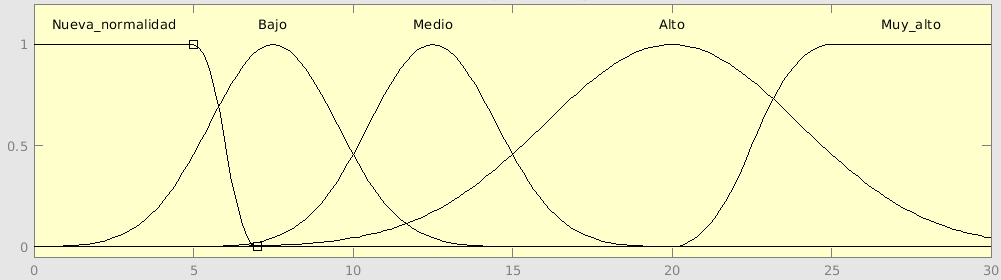
\includegraphics[width=300px]{img/camas_UCI.png}
      \caption{UCI}
      \label{UCI}
    \end{figure}

    \item \textbf{Ocupación de camas de hospitalización por casos de COVID-19} (Camas):  Número de camas de hospitalización ocupadas por casos de COVID / Número total de camas de hospitalización en funcionamiento. Sus posibles valores son: \textit{Muy Bajo}, \textit{Bajo} \textit{Medio }, {\textit{Alto}} y {\textit{Muy Alto}}. La figura~\ref{Camas} muestra los intervalos de cada uno de los posibles valores de forma gráfica.
    
    \begin{figure}[!h]
      \centering
      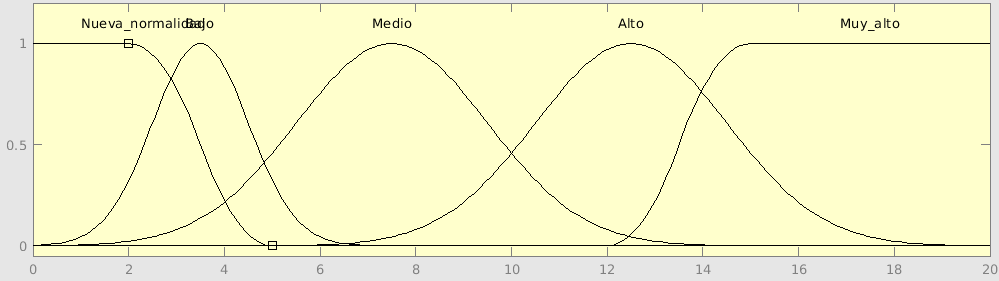
\includegraphics[width=300px]{img/ocupacion_camas.png}
      \caption{Camas}
      \label{Camas}
    \end{figure}

    \end{itemize}

\subsection{Variable de salida}

Se establece como variable de salida el hecho de confinar o no una población en función de tres niveles diferenciados. \textit{No confinar, Considerar el confinamiento y Sí confinar}. Se hace hincapié en el sentido del valor \textit{Considerar el confinamiento} que indica a los responsables de confinar un territorio que sería recomendable hacerlo atendiendo únicamente a razones sanitarias, pero que existe capacidad de discusión de otro tipo de medidas que no perjudiquen en esa medida a los sectores productivos de la población.  La figura 7 muestra los intervalos de cada uno de los posibles valores de forma gráfica.

\begin{figure}[!h]
  \centering
  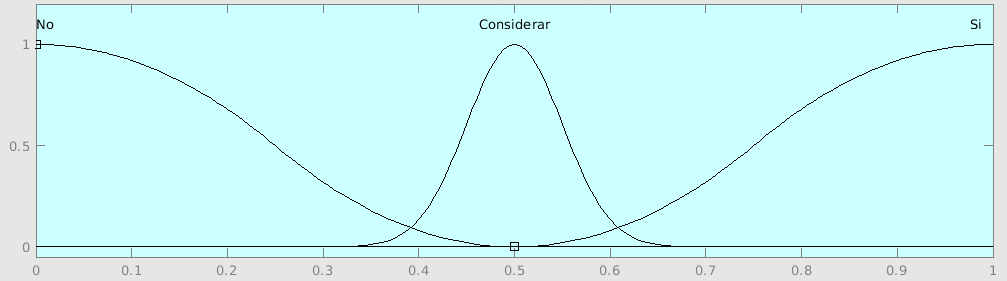
\includegraphics[width=300px]{img/confinar.png}
  \caption{Confinar}
\end{figure}

\subsection{Reglas}

Todas las reglas son del tipo \textit{AND} menos la primera que es del tipo \textit{OR}.

\begin{center}
\begin{tabular}{c|c|c|c|c|c|c|c|c|}
  \cline{2-9}
                                & IA-14 & IA-7 & IA-14 65 & IA-7 65 & PDI & UCI & Camas & \textbf{Confinar} \\ \hline
\multicolumn{1}{|c|}{Regla 1} & \begin{tabular}[c]{@{}c@{}}Muy\\ alto\end{tabular} & \begin{tabular}[c]{@{}c@{}}Muy\\ alto\end{tabular} & \begin{tabular}[c]{@{}c@{}}Muy\\ alto\end{tabular} & \begin{tabular}[c]{@{}c@{}}Muy\\ alto\end{tabular} & \begin{tabular}[c]{@{}c@{}}Muy\\ alto\end{tabular} & \begin{tabular}[c]{@{}c@{}}Muy\\ alto\end{tabular} & \begin{tabular}[c]{@{}c@{}}Muy\\ alto\end{tabular}& Sí \\ \hline
\multicolumn{1}{|c|}{Regla 2} & Medio & Medio & - & - & - & - & Alto & Si \\ \hline
\multicolumn{1}{|c|}{Regla 3} & Alto & Alto & Alto & Alto & Alto & Alto & Alto & Sí \\ \hline
\multicolumn{1}{|c|}{Regla 4} & \begin{tabular}[c]{@{}c@{}}Nueva\\ norm.\end{tabular} & \begin{tabular}[c]{@{}c@{}}Nueva\\ norm.\end{tabular} & \begin{tabular}[c]{@{}c@{}}Nueva\\ norm.\end{tabular} & \begin{tabular}[c]{@{}c@{}}Nueva\\ norm.\end{tabular} & \begin{tabular}[c]{@{}c@{}}Nueva\\ norm.\end{tabular} & \begin{tabular}[c]{@{}c@{}}Nueva\\ norm.\end{tabular} & \begin{tabular}[c]{@{}c@{}}Nueva\\ norm.\end{tabular} & No \\ \hline
\multicolumn{1}{|c|}{Regla 5} & Bajo & Alto & - & - & - & - & - & Sí \\ \hline
\multicolumn{1}{|c|}{Regla 6} & Bajo & Medio & - & - & - & - & - & Considerar \\ \hline
\multicolumn{1}{|c|}{Regla 7} & Medio & Medio & - & - & - & Alto & - & Sí \\ \hline
\multicolumn{1}{|c|}{Regla 8} & - & - & - & - & - & Bajo & Bajo & No \\ \hline
\multicolumn{1}{|c|}{Regla 9} & Medio & Medio & Alto & Alto & - & - & - & Sí \\ \hline
\multicolumn{1}{|c|}{Regla 10} & Medio & Medio & - & - & - & \begin{tabular}[c]{@{}c@{}}Nueva\\ norm.\end{tabular} & \begin{tabular}[c]{@{}c@{}}Nueva\\ norm.\end{tabular} & No \\ \hline
\multicolumn{1}{|c|}{Regla 11} & Bajo & Bajo & Bajo & Bajo & Bajo & Bajo & Bajo & No \\ \hline
\multicolumn{1}{|c|}{Regla 12} & Alto & Bajo & - & - & - & - & - & No \\ \hline
\multicolumn{1}{|c|}{Regla 13} & - & - & Bajo & Alto & - & - & - & Considerar \\ \hline
\multicolumn{1}{|c|}{Regla 14} & - & - & - & - & Alto & - & - & Considerar \\ \hline
\end{tabular}
\end{center}



\section{Sistema borroso: Prueba PCR}

Este segundo sistema basado en lógica borrosa debe decidir si dado un paciente, es o no candidato a que se le realice una prueba PCR. Para ello, se definen una serie de variables de entrada obtenidas del \textit{Ministerio de Sanidad}\cite{paciente}, se ha decidido seleccionar aquellas que se cree que son más relevantes. Además, se establece la variable de salida y por último las reglas para la toma de decisiones.

\vspace{2mm}

Un sistema que consiga resolver este problema de forma eficaz sería de gran ayuda en los centros médicos, ya que aliviaría la carga de trabajo de los médicos y sería de utilidad a la hora de tomar decisiones sobre clasos inconcluyentes.


\subsection{Variables de entrada}

Las entradas del sistema seleccionadas son:

\begin{itemize}
  \item \textbf{Días desde primeros síntomas} (DDPS) figura~\ref{DDPS}: representa el número de días que el paciente lleva con síntomas relacionados con el \textit{COVID-19}. Sus posibles valores son: \textit{Pocos}, \textit{Medios} y \textit{Muchos}.

  \begin{figure}[!h]
      \centering
      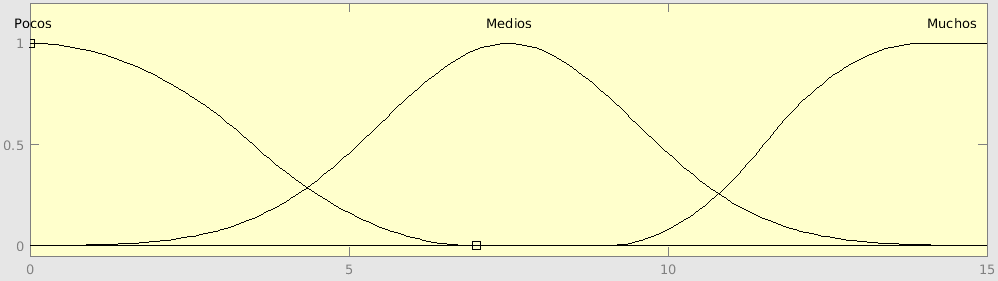
\includegraphics[width=300px]{img/dias_primeros_sintomas.png}
      \caption{DDPS}
      \label{DDPS}
  \end{figure}

  \item \textbf{Prueba rápida} figura~\ref{PR}: si el paciente ha dado positivo o negativo en una prueba rápida, por lo tanto sus valores son solo \textit{Sí} o \textit{No}. Si al paciente no se le ha realizado ninguna prueba rápida se representará con un 0,5.

  \begin{figure}[!h]
      \centering
      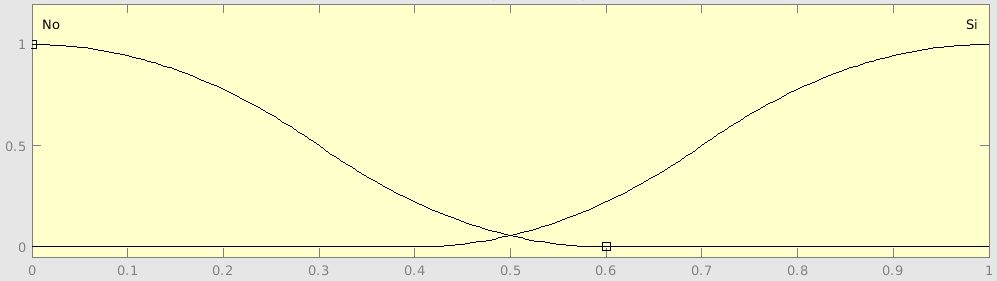
\includegraphics[width=300px]{img/prueba_rapida.png}
      \caption{Prueba rápida}
      \label{PR}
  \end{figure}

  \item \textbf{PCR} figura~\ref{PCR}: si el paciente ha dado positivo o negativo en una prueba PCR, al igual que en la variable anterior, sus valores son solo \textit{Sí} o \textit{No}. Si al paciente no se le ha realizado ninguna PCR se representará con un 0,5.

  \begin{figure}[!h]
      \centering
      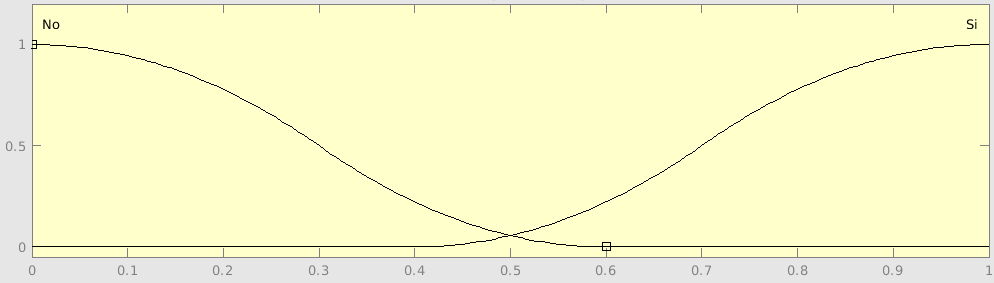
\includegraphics[width=300px]{img/PCR.png}
      \caption{PCR}
      \label{PCR}
  \end{figure}

  \item \textbf{UCI} figura~\ref{UCI}: si el paciente tiene que ser ingresado en la UCI, posibles valores: \textit{Sí} o \textit{No}.

  \begin{figure}[!h]
      \centering
      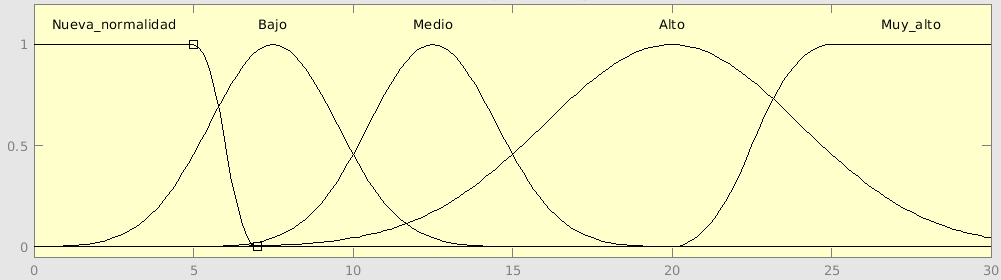
\includegraphics[width=300px]{img/UCI.png}
      \caption{UCI}
      \label{UCI}
  \end{figure}

  \item \textbf{Sospecha clínica} figura~\ref{SC}: creencia del médico de si el paciente puede tener o no el \textit{COVID-19}. Toma valores de \textit{Baja}, \textit{Media} y \textit{Alta}.

  \begin{figure}[!h]
      \centering
      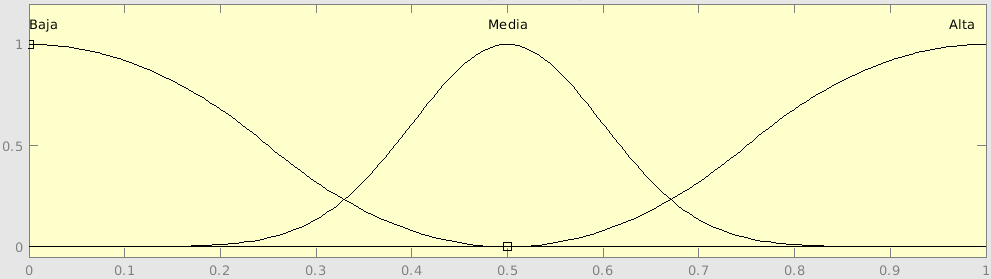
\includegraphics[width=300px]{img/sospecha_clinica.png}
      \caption{Sospecha clínica}
      \label{SC}
  \end{figure}

  \item \textbf{Días desde contacto positivo} (DDCP) figura~\ref{DDCP}: representa el número de días desde que el paciente ha estado en contacto con una persona positiva de \textit{COVID-19}. Sus posibles valores son: \textit{Pocos}, \textit{Medios} y \textit{Muchos}.

  \begin{figure}[!h]
      \centering
      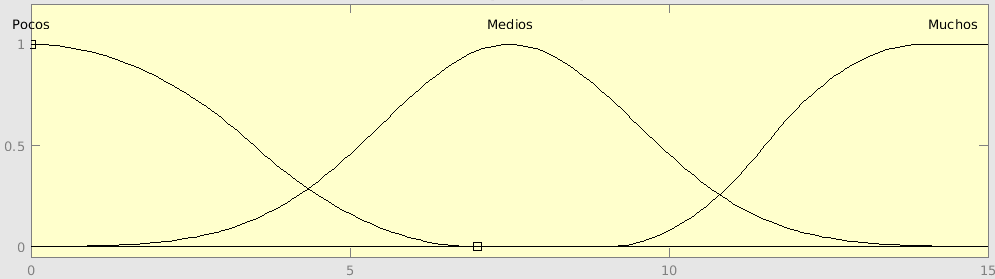
\includegraphics[width=300px]{img/dias_desde_cntcto_positivo.png}
      \caption{DDCP}
      \label{DDCP}
  \end{figure}

  \item \textbf{Síntomas} figura~\ref{Sintomas}: indica el número de síntomas de \textit{COVID-19} que tiene el paciente. Puede tomar valores de \textit{Ninguno}, \textit{Alguno}, \textit{Varios} y \textit{Todos}.

  \begin{figure}[!h]
      \centering
      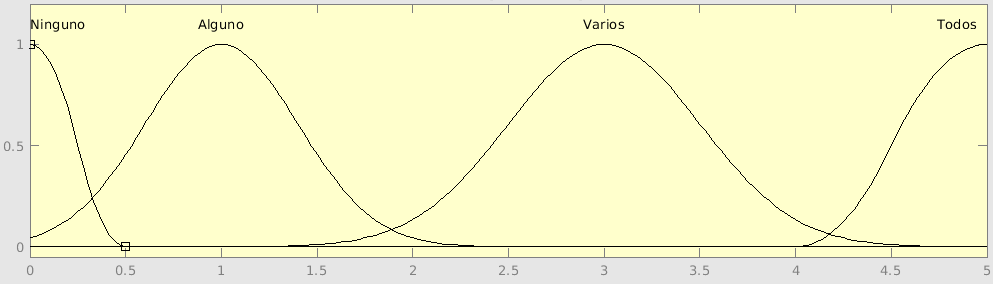
\includegraphics[width=300px]{img/sintomas.png}
      \caption{Síntomas}
      \label{Sintomas}
  \end{figure}

  \item \textbf{Uso mascarilla con no convivientes} (UMNC) figura~\ref{UMNC}: si el paciente usa regularmente la mascarilla cuando se encuentra con personas con las que no convive, sus valores son solo \textit{Sí} o \textit{No}.

  \begin{figure}[!h]
      \centering
      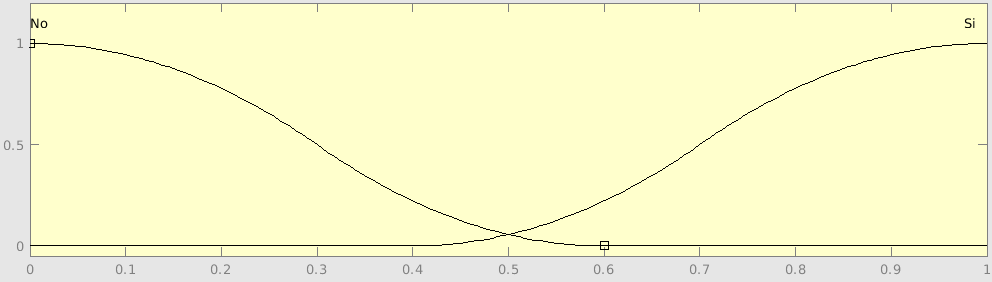
\includegraphics[width=300px]{img/uso_mascarilla.png}
      \caption{UMNC}
      \label{UMNC}
  \end{figure}

\end{itemize}



\subsection{Variable de salida}

Como la decisión a tomar es si se debe realizar o no una prueba PCR, la salida del sistema es la certeza que se tiene de si se debe realizar la prueba o no al paciente. Sus valores son \textit{Sí} o \textit{No} (figura~\ref{realizarPCR}).

\begin{figure}[!h]
    \centering
    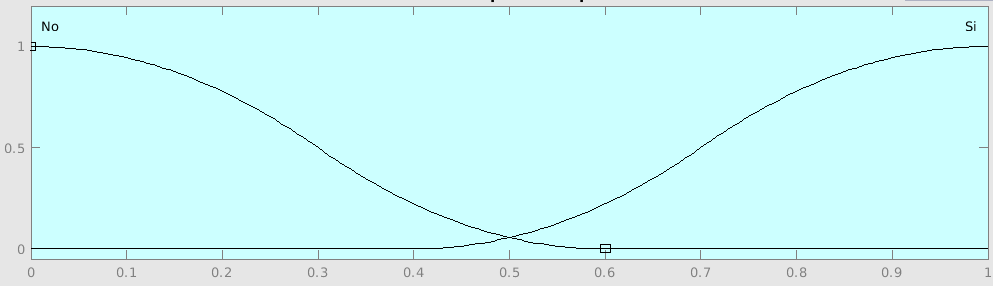
\includegraphics[width=300px]{img/realizar_pcr.png}
    \caption{Realizar PCR}
    \label{realizarPCR}
\end{figure}



\subsection{Reglas}

Todas las reglas son del tipo \textit{AND}. Para las 7 primeras reglas se ha tomado como referencia la información del \textit{Ministerio de Sanidad}\cite{paciente}, las siguientes son creadas bajo el criterio de los autores con el fin de completar la funcionalidad del sistema.

\begin{center}
  \begin{adjustwidth}{-1.3cm}{}
\begin{tabular}{c|c|c|c|c|c|c|c|c|c|}
  \cline{2-10}
                                & DDPS & \begin{tabular}[c]{@{}c@{}}Prueba\\ Rápida\end{tabular} & PCR & UCI & \begin{tabular}[c]{@{}c@{}}Sospecha\\ Clínica\end{tabular} & DDCP & Síntomas & UMNC & \begin{tabular}[c]{@{}c@{}}\textbf{Realizar}\\ \textbf{PCR}\end{tabular} \\ \hline
\multicolumn{1}{|c|}{Regla 1} & \textit{Not} Pocos & - & - & - & - & - & - & - & Sí \\ \hline
\multicolumn{1}{|c|}{Regla 2} & - & - & No & - & Alta & - & - & - & Sí \\ \hline
\multicolumn{1}{|c|}{Regla 3} & - & No & - & - & Alta & - & - & - & Sí \\ \hline
\multicolumn{1}{|c|}{Regla 4} & \textit{Not} Pocos & No & - & - & - & - & - & - & Sí \\ \hline
\multicolumn{1}{|c|}{Regla 5} & - & - & Sí & - & - & - & - & - & Sí \\ \hline
\multicolumn{1}{|c|}{Regla 6} & - & - & - & - & - & Muchos & Ninguno & - & No \\ \hline
\multicolumn{1}{|c|}{Regla 7} & - & - & - & - & - & \textit{Not} Mucho & Ninguno & Sí & No \\ \hline
\multicolumn{1}{|c|}{Regla 8} & Pocos & - & - & - & \textit{Not} Alta & - & - & - & No \\ \hline
\multicolumn{1}{|c|}{Regla 9} & - & Sí & - & - & Baja & - & - & - & Sí \\ \hline
\multicolumn{1}{|c|}{Regla 10} & - & - & - & - & - & \textit{Not} Muchos & \textit{Not} Ninguno & No & Sí \\ \hline
\multicolumn{1}{|c|}{Regla 11} & \textit{Not} Pocos & - & - & - & - & - & Todos & - & Sí \\ \hline
\multicolumn{1}{|c|}{Regla 12} & - & No & - & - & Baja & - & - & - & No \\ \hline
\multicolumn{1}{|c|}{Regla 13} & - & No & - & - & - & - & Varios & - & No \\ \hline
\multicolumn{1}{|c|}{Regla 14} & - & - & - & - & \textit{Not} Alta & - & Alguno & - & No \\ \hline
\end{tabular}
\end{adjustwidth}
\end{center}





\section{Validación del sistema}

  \subsection{Confinamiento}
    \begin{center}
      \hspace{-13mm}
    \begin{tabular}{c|c|c|c|c|c|c|c|c|}
      \cline{2-9}
                                    & IA-14 & IA-7 & IA-14 65 & IA-7 65 & PDI & UCI & Camas & \textbf{Prob. Confinar} \\ \hline
    \multicolumn{1}{|c|}{Prueba 1} & 300 & 200 & 200 & 100 & 23 & 28 & 18 & 0.8571 \\ \hline
    \multicolumn{1}{|c|}{Prueba 2} & 400 & 150 & 150 & 200 & 29 & 23 & 15 & 0.8571 \\ \hline
    \multicolumn{1}{|c|}{Prueba 3} & 160 & 80 & 110 & 55 & 11 & 16 & 11 & 0.6936 \\ \hline
    \multicolumn{1}{|c|}{Prueba 4} & 240 & 120 & 140 & 70 & 14 & 23 & 14 & 0.7550 \\ \hline
    \multicolumn{1}{|c|}{Prueba 5} & 55 & 30 & 60 & 35 & 8 & 11 & 6 & 0.5427 \\ \hline
    \multicolumn{1}{|c|}{Prueba 6} & 60 & 40 & 50 & 40 & 9 & 14 & 8 & 0.6622 \\ \hline
    \multicolumn{1}{|c|}{Prueba 7} & 30 & 15 & 30 & 13 & 5 & 7 & 3 & 0.1709 \\ \hline
    \multicolumn{1}{|c|}{Prueba 8} & 40 & 20 & 40 & 20 & 7 & 9 & 4 & 0.2129 \\ \hline
    \multicolumn{1}{|c|}{Prueba 9} & 5 & 3 & 2 & 2 & 1 & 2 & 0 & 0.1458 \\ \hline
    \multicolumn{1}{|c|}{Prueba 10} & 20 & 9 & 15 & 9 & 3 & 4 & 2 & 0.2158 \\ \hline
    \end{tabular}
    \end{center}

    \vspace{2mm}

    \begin{center}
      \hspace{-13mm}
    \begin{tabular}{c|c|c|c|c|c|c|c|c|}
      \cline{2-9}
                                    & IA-14 & IA-7 & IA-14 65 & IA-7 65 & PDI & UCI & Camas & \textbf{Prob. Confinar} \\ \hline
    \multicolumn{1}{|c|}{Prueba 1} & 100 & 100 & 15 & 60 & 8 & 7 & 12 & 0.7755 \\ \hline
    \multicolumn{1}{|c|}{Prueba 2} & 5 & 21 & 125 & 5 & 2 & 25 & 4 & 0.8164 \\ \hline
    \multicolumn{1}{|c|}{Prueba 3} & 200 & 25 & 75 & 20 & 4 & 13 & 16 & 0.6410 \\ \hline
    \end{tabular}
    \end{center}

  \subsection{Prueba PCR}
    
    \begin{center}
    \begin{tabular}{c|c|c|c|c|c|c|c|c|c|}
      \cline{2-10}
                                    & DDPS & \begin{tabular}[c]{@{}c@{}}Prueba\\ Rápida\end{tabular} & PCR & UCI & \begin{tabular}[c]{@{}c@{}}Sospecha\\ Clínica\end{tabular} & DDCP & Síntomas & UMNC & \begin{tabular}[c]{@{}c@{}}\textbf{Prob.}\\ \textbf{Realizar}\\ \textbf{PCR}\end{tabular} \\ \hline
    \multicolumn{1}{|c|}{Prueba 1} & 1.5 & 0.5 & 0.5 & 0 & 0.1 & 1.5 & 0.5 & 0.1 & 0.5033 \\ \hline
    \multicolumn{1}{|c|}{Prueba 2} & 3 & 0.5 & 0.5 & 0 & 0.2 & 3 & 1 & 0.2 & 0.472 \\ \hline
    \multicolumn{1}{|c|}{Prueba 3} & 4.5 & 0.5 & 0.5 & 0 & 0.3 & 4.5 & 1.5 & 0.3 & 0.5633 \\ \hline
    \multicolumn{1}{|c|}{Prueba 4} & 6 & 0 & 0.5 & 0 & 0.4 & 0.6 & 2 & 0.4 & 0.7228 \\ \hline
    \multicolumn{1}{|c|}{Prueba 5} & 7.5 & 0.5 & 0 & 0 & 0.5 & 7,5 & 2.5 & 0.5 & 0.7807 \\ \hline
    \multicolumn{1}{|c|}{Prueba 6} & 9 & 0.5 & 1 & 0 & 0.5 & 9 & 3 & 0.6 & 0.7807 \\ \hline
    \multicolumn{1}{|c|}{Prueba 7} & 10.5 & 0.5 & 1 & 1 &0.6 & 10.5 & 3.5 & 0.7 & 0.7807 \\ \hline
    \multicolumn{1}{|c|}{Prueba 8} & 12 & 1 & 0.5 & 0 & 0.7 & 12 & 4 & 0.80 & 0.8279 \\ \hline
    \multicolumn{1}{|c|}{Prueba 9} & 13 & 1 & 0.5 & 1 & 0.8 & 13.5 & 4.5 & 0.9 & 0.8279 \\ \hline
    \multicolumn{1}{|c|}{Prueba 10} & 15 & 1 & 0.5 & 0 & 0.1 & 0.0 & 0.0 & 0.0 & 0.8279 \\ \hline
    \multicolumn{1}{|c|}{Prueba 11} & 10 & 0 & 0.5 & 0 & 0.1 & 0.0 & 0.0 & 0.0 & 0.7245 \\ \hline
    \multicolumn{1}{|c|}{Prueba 12} & 8 & 1 & 0.5 & 0 & 0.1 & 0.0 & 0.0 & 0.0 & 0.8279 \\ \hline
    \multicolumn{1}{|c|}{Prueba 13} & 4 & 1 & 0.5 & 0 & 0.1 & 0.0 & 0.0 & 0.0 & 0.7617 \\ \hline
    \multicolumn{1}{|c|}{Prueba 14} & 0 & 1 & 0.5 & 0 & 0 & 5 & 0 & 1 & 0.5 \\ \hline
    \multicolumn{1}{|c|}{Prueba 15} & 10 & 0.5 & 1 & 0 & 0.2 & 15 & 1 & 0.9 & 0.5 \\ \hline
    \multicolumn{1}{|c|}{Prueba 16} & 10 & 0.5 & 1 & 0 & 0.8 & 12 & 3 & 0.9 & 0.7807 \\ \hline
    \multicolumn{1}{|c|}{Prueba 17} & 2 & 0.5 & 0.5 & 1 & 0.5 & 6 & 3 & 0.8 & 0.5146 \\ \hline
    \multicolumn{1}{|c|}{Prueba 18} & 2 & 0.5 & 0.5 & 0 & 0.3 & 2 & 0 & 0.9 & 0.2947 \\ \hline
    \multicolumn{1}{|c|}{Prueba 19} & 15 & 1 & 1 & 0 & 0.2 & 7 & 1 & 0.75 & 0.5 \\ \hline
    \multicolumn{1}{|c|}{Prueba 20} & 7 & 0 & 0 & 0 & 0.4 & 9 & 2 & 0.6 & 0.7245 \\ \hline
    \multicolumn{1}{|c|}{Prueba 21} & 14 & 0.5 & 0 & 0 & 0.4 & 7 & 5 & 0.1 & 0.7807 \\ \hline
    \multicolumn{1}{|c|}{Prueba 22} & 2 & 1 & 0.5 & 1 & 0.9 & 3 & 0 & 0.8 & 0.5228 \\ \hline
    \multicolumn{1}{|c|}{Prueba 23} & 7 & 0 & 0 & 0 & 0.6 & 14 & 1 & 0.2 & 0.5052 \\ \hline
    \end{tabular}
    \end{center}
  
  \subsection{Analisis de los resultados}

\section{Conclusiones}

  A lo largo del desarrollo de esta práctica se ha profundizado en la técnica de \textit{Lógica Difusa}, la misma presenta un enfoque bien diferenciado de otras técnicas de Inteligencia Artificial, puesto que permite la resolución de problemas para los cuales no existe una alternativa eficiente que sea \textbf{capaz de trabajar con la incertidumbre humana}. Por todo ello, esta práctica resulta de utilidad si se pretende introducirse en ese mundo de manera sucinta. Sin embargo, también impone la resolución de unos retos que deben ser solucionados si se pretende afrontar aplicaciones reales. 
  
  \vspace{2mm}
  
  Entre las principales desventajas o retos que acarrea esta técnica está la \textbf{dificultad de establecer reglas} exactas así como los distintos intervalos de cada una de las variables para disponer de un sistema lo más fiel posible. Esto es así debido a las propias características de la lógica difusa, puesto que al ser capaz de trabajar con la incertidumbre humana pierde la capacidad de detectar patrones inadvertidos a los humanos como sí pueden encontrar, por ejemplo, las redes de neuronas.
      
  \vspace{2mm}
  
  
  Otra piedra en el camino a la hora de realizar una tarea de lógica difusa con éxito consiste en encontrar una \textbf{fuente fiable de conocimiento} para posibilitar la creación de reglas y casos de prueba, lo cual se pone de manifiesto en situaciones tan caóticas como la epidemia de \textit{SARS-CoV-2}. 
  
  \vspace{2mm}
  
  A pesar de sus múltiples desventajas,la lógica difusa es una técnica especialmente útil especialmente si se contrasta con otras técnicas conocidas como caja negra, es \textbf{extremadamente fácil obtener explicaciones} sobre los resultados en base a las reglas activadas.
  
  \vspace{2mm}
  
  A modo de conclusión se destaca la importancia de disponer de distintas herramientas de Inteligencia Artificial que permitan su aplicación en situaciones bien diferenciadas, permitiendo de esta manera seleccionar la técnica que mejor se adapte a lo que se pretende obtener en cada momento. Puesto que no existen técnicas universales la tarea de un ingeniero experto en Inteligencia Artificial debe ser la seleccionar el conjunto de técnicas que mejor funcione en cada momento.
  
\clearpage 

\bibliographystyle{ieeetr}
\bibliography{bibliografia.bib}


\end{document}
